\documentclass[12pt]{article}
\usepackage{graphicx}
\usepackage{float}
\usepackage{geometry}
\usepackage{fontspec}
\usepackage{hyperref}

\hypersetup{
colorlinks=true,
linkcolor=blue,
filecolor=blue,      
urlcolor=blue,
citecolor=cyan,
}

\geometry{a4paper, left=2.54cm, right=2.54cm, top=2.54cm, bottom=2.54cm}
\setmainfont{Times New Roman}
\linespread{1.5}

% COVER

\begin{document}
\begin{titlepage}
    \centering
    
\includegraphics[width=0.6\textwidth]{Logo.png}\par\vspace{1cm}
    \vspace{1cm}
    {\scshape\LARGE Title\par}
    \vspace{2.5cm}
    {\Large Coursework 3: ?\par}
    \vspace{6cm}
    {\Large Name\par}
    \vspace{0.5cm}
    {\Large email\par}
    \vfill
    {\Large April 2023\par}
\end{titlepage}

% MAIN BODY
\section{Introduction and Motivation}

abc
\\ \hspace*{\fill} \\
abc
\\ \hspace*{\fill} \\
abc

\begin{figure}[H]
\centering
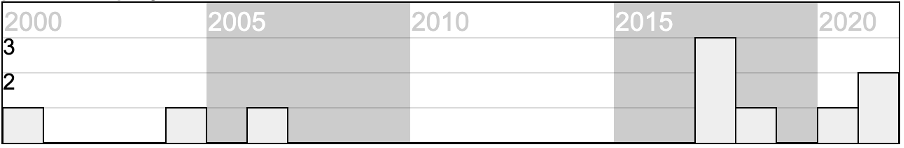
\includegraphics[width=0.7\textwidth]{meta-data.png}
\caption{Figure1} 
\end{figure}

\noindent abc

\begin{figure}[H]
\centering
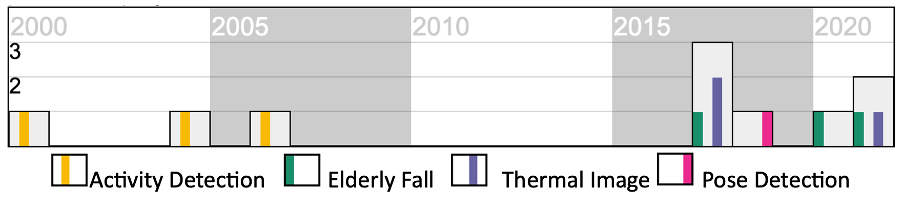
\includegraphics[width=0.7\textwidth]{supplementary-figure.png}
\caption{Figure2} 
\end{figure}

\noindent abc

\subsection{Field Challenges}

abc
\\ \hspace*{\fill} \\
abc
\\ \hspace*{\fill} \\
abc

\subsection{Survey Scope}

abc

\subsection{Search Methodology}

abc

\begin{figure}[H]
\centering
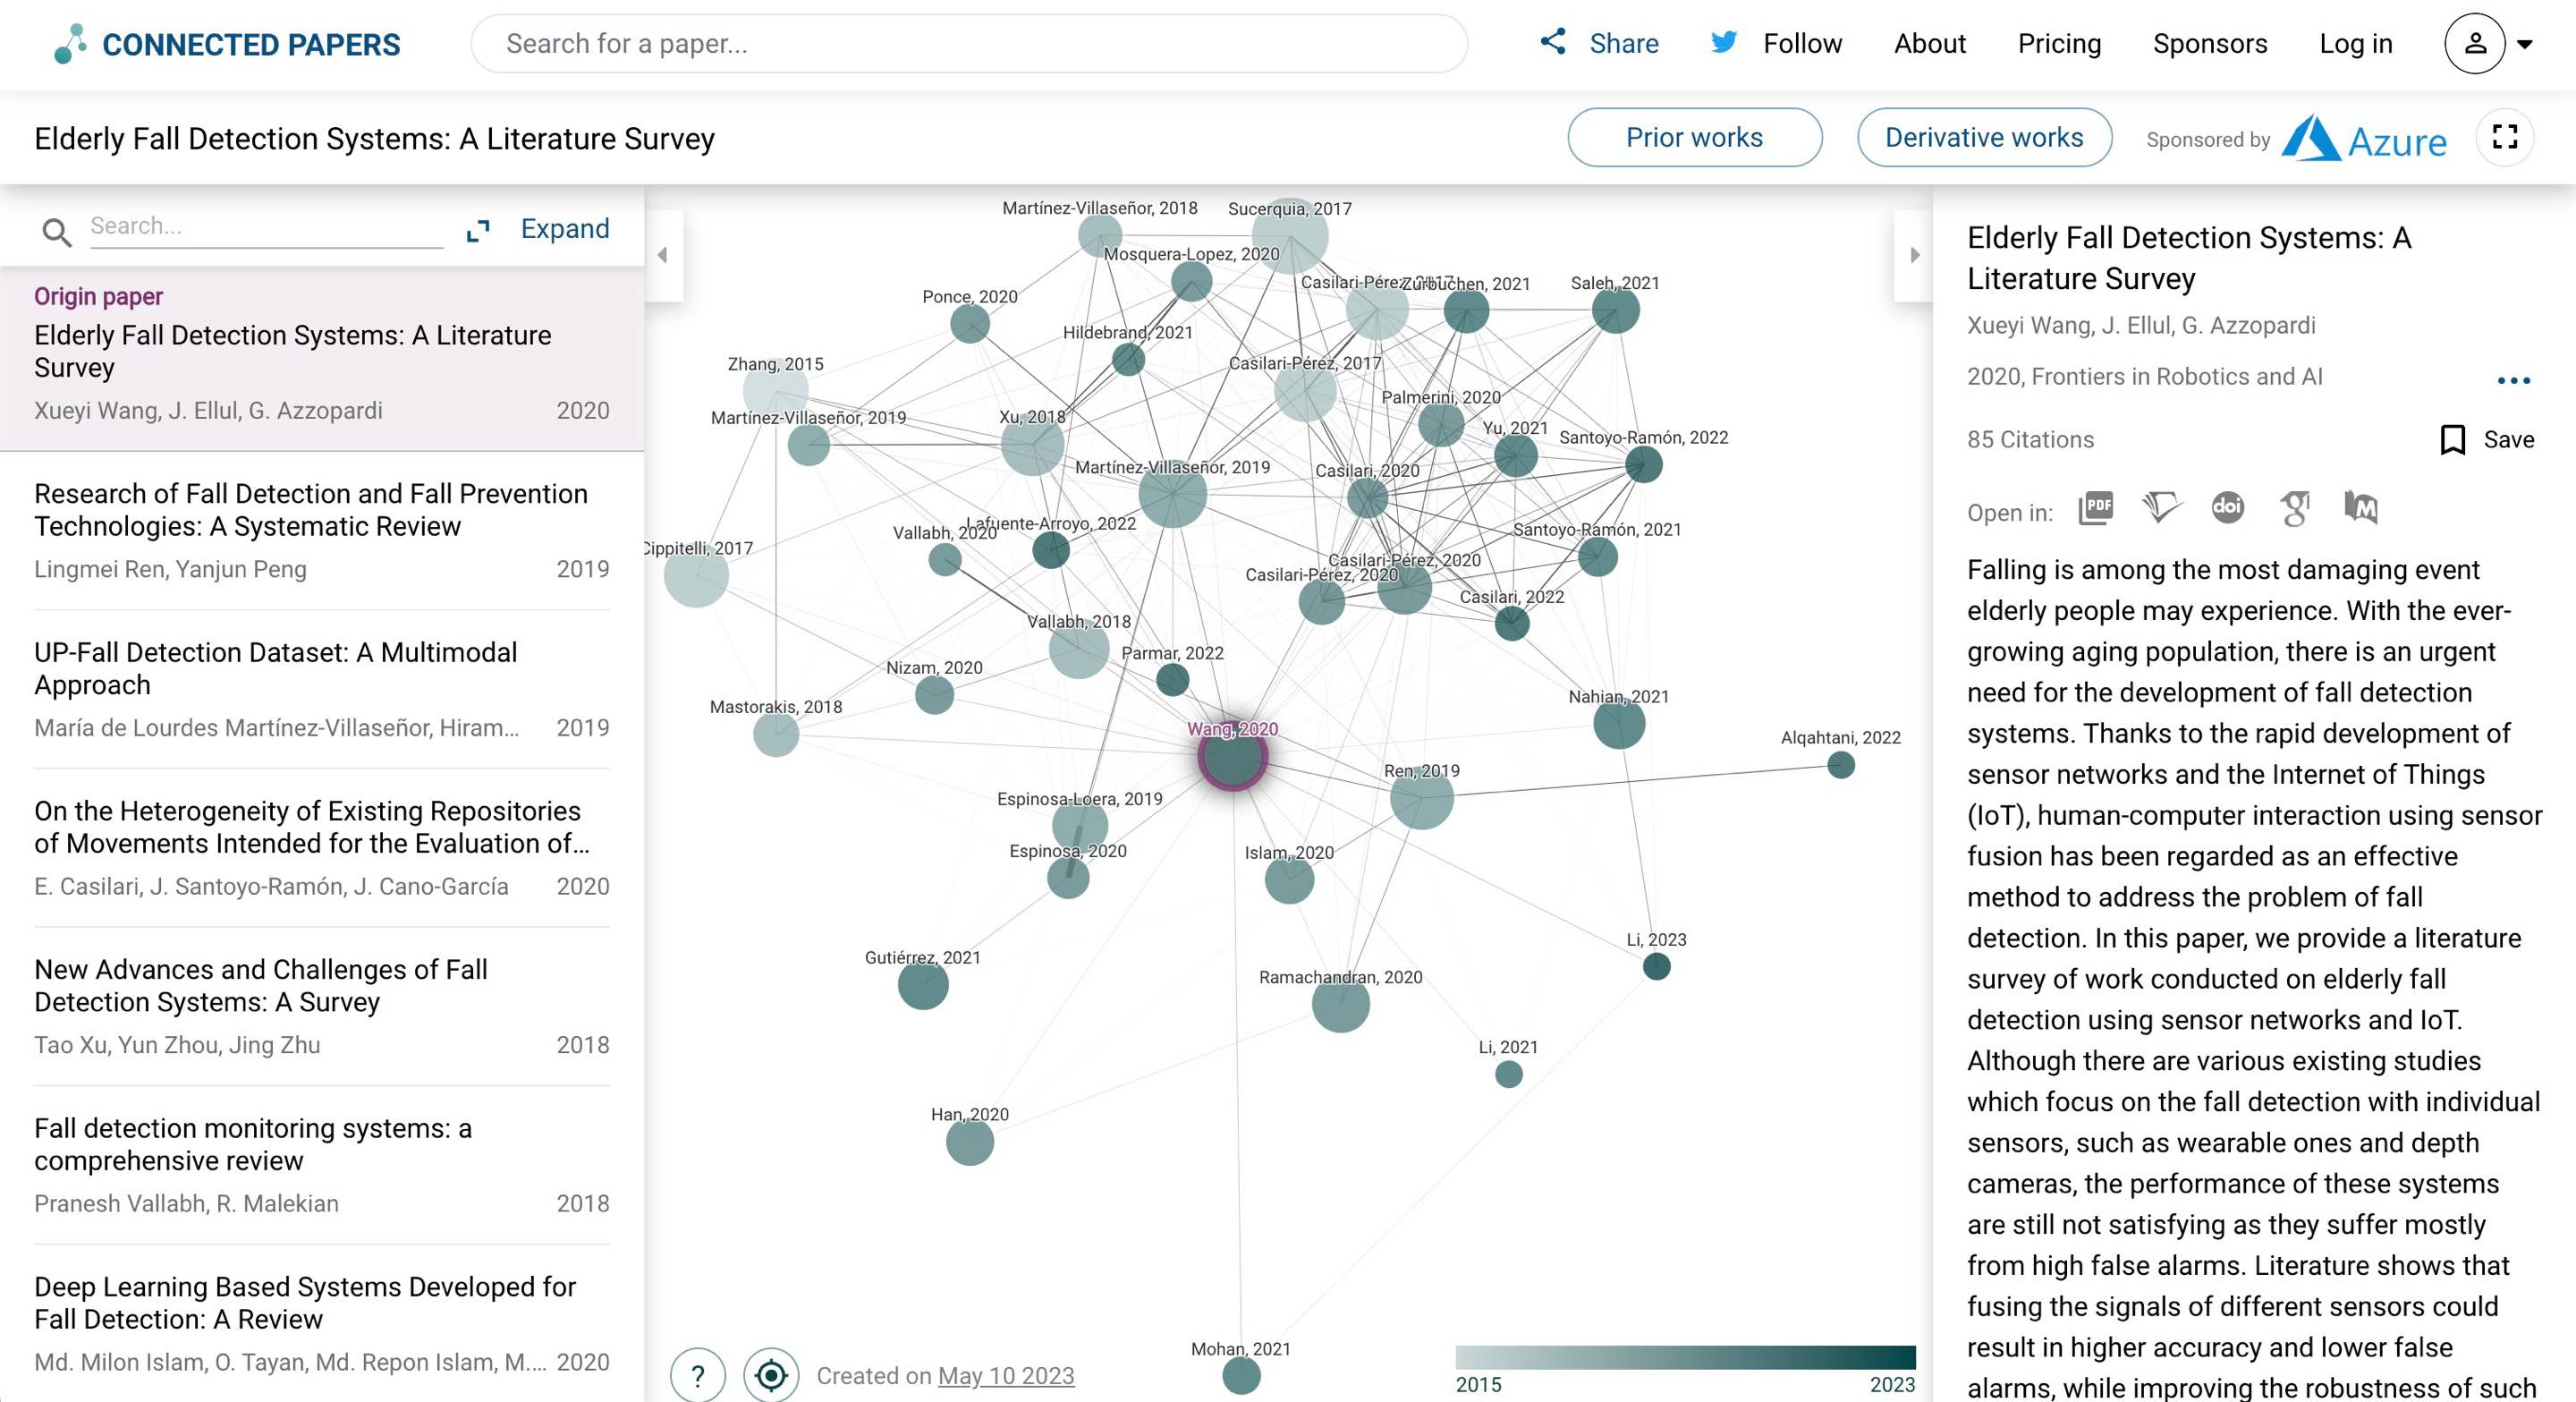
\includegraphics[width=1\textwidth]{connected-paper.pic.jpg}
\caption{Figure3} 
\end{figure}

\subsection{Classification of Literature and Organization}

abc

\begin{figure}[H]
\centering
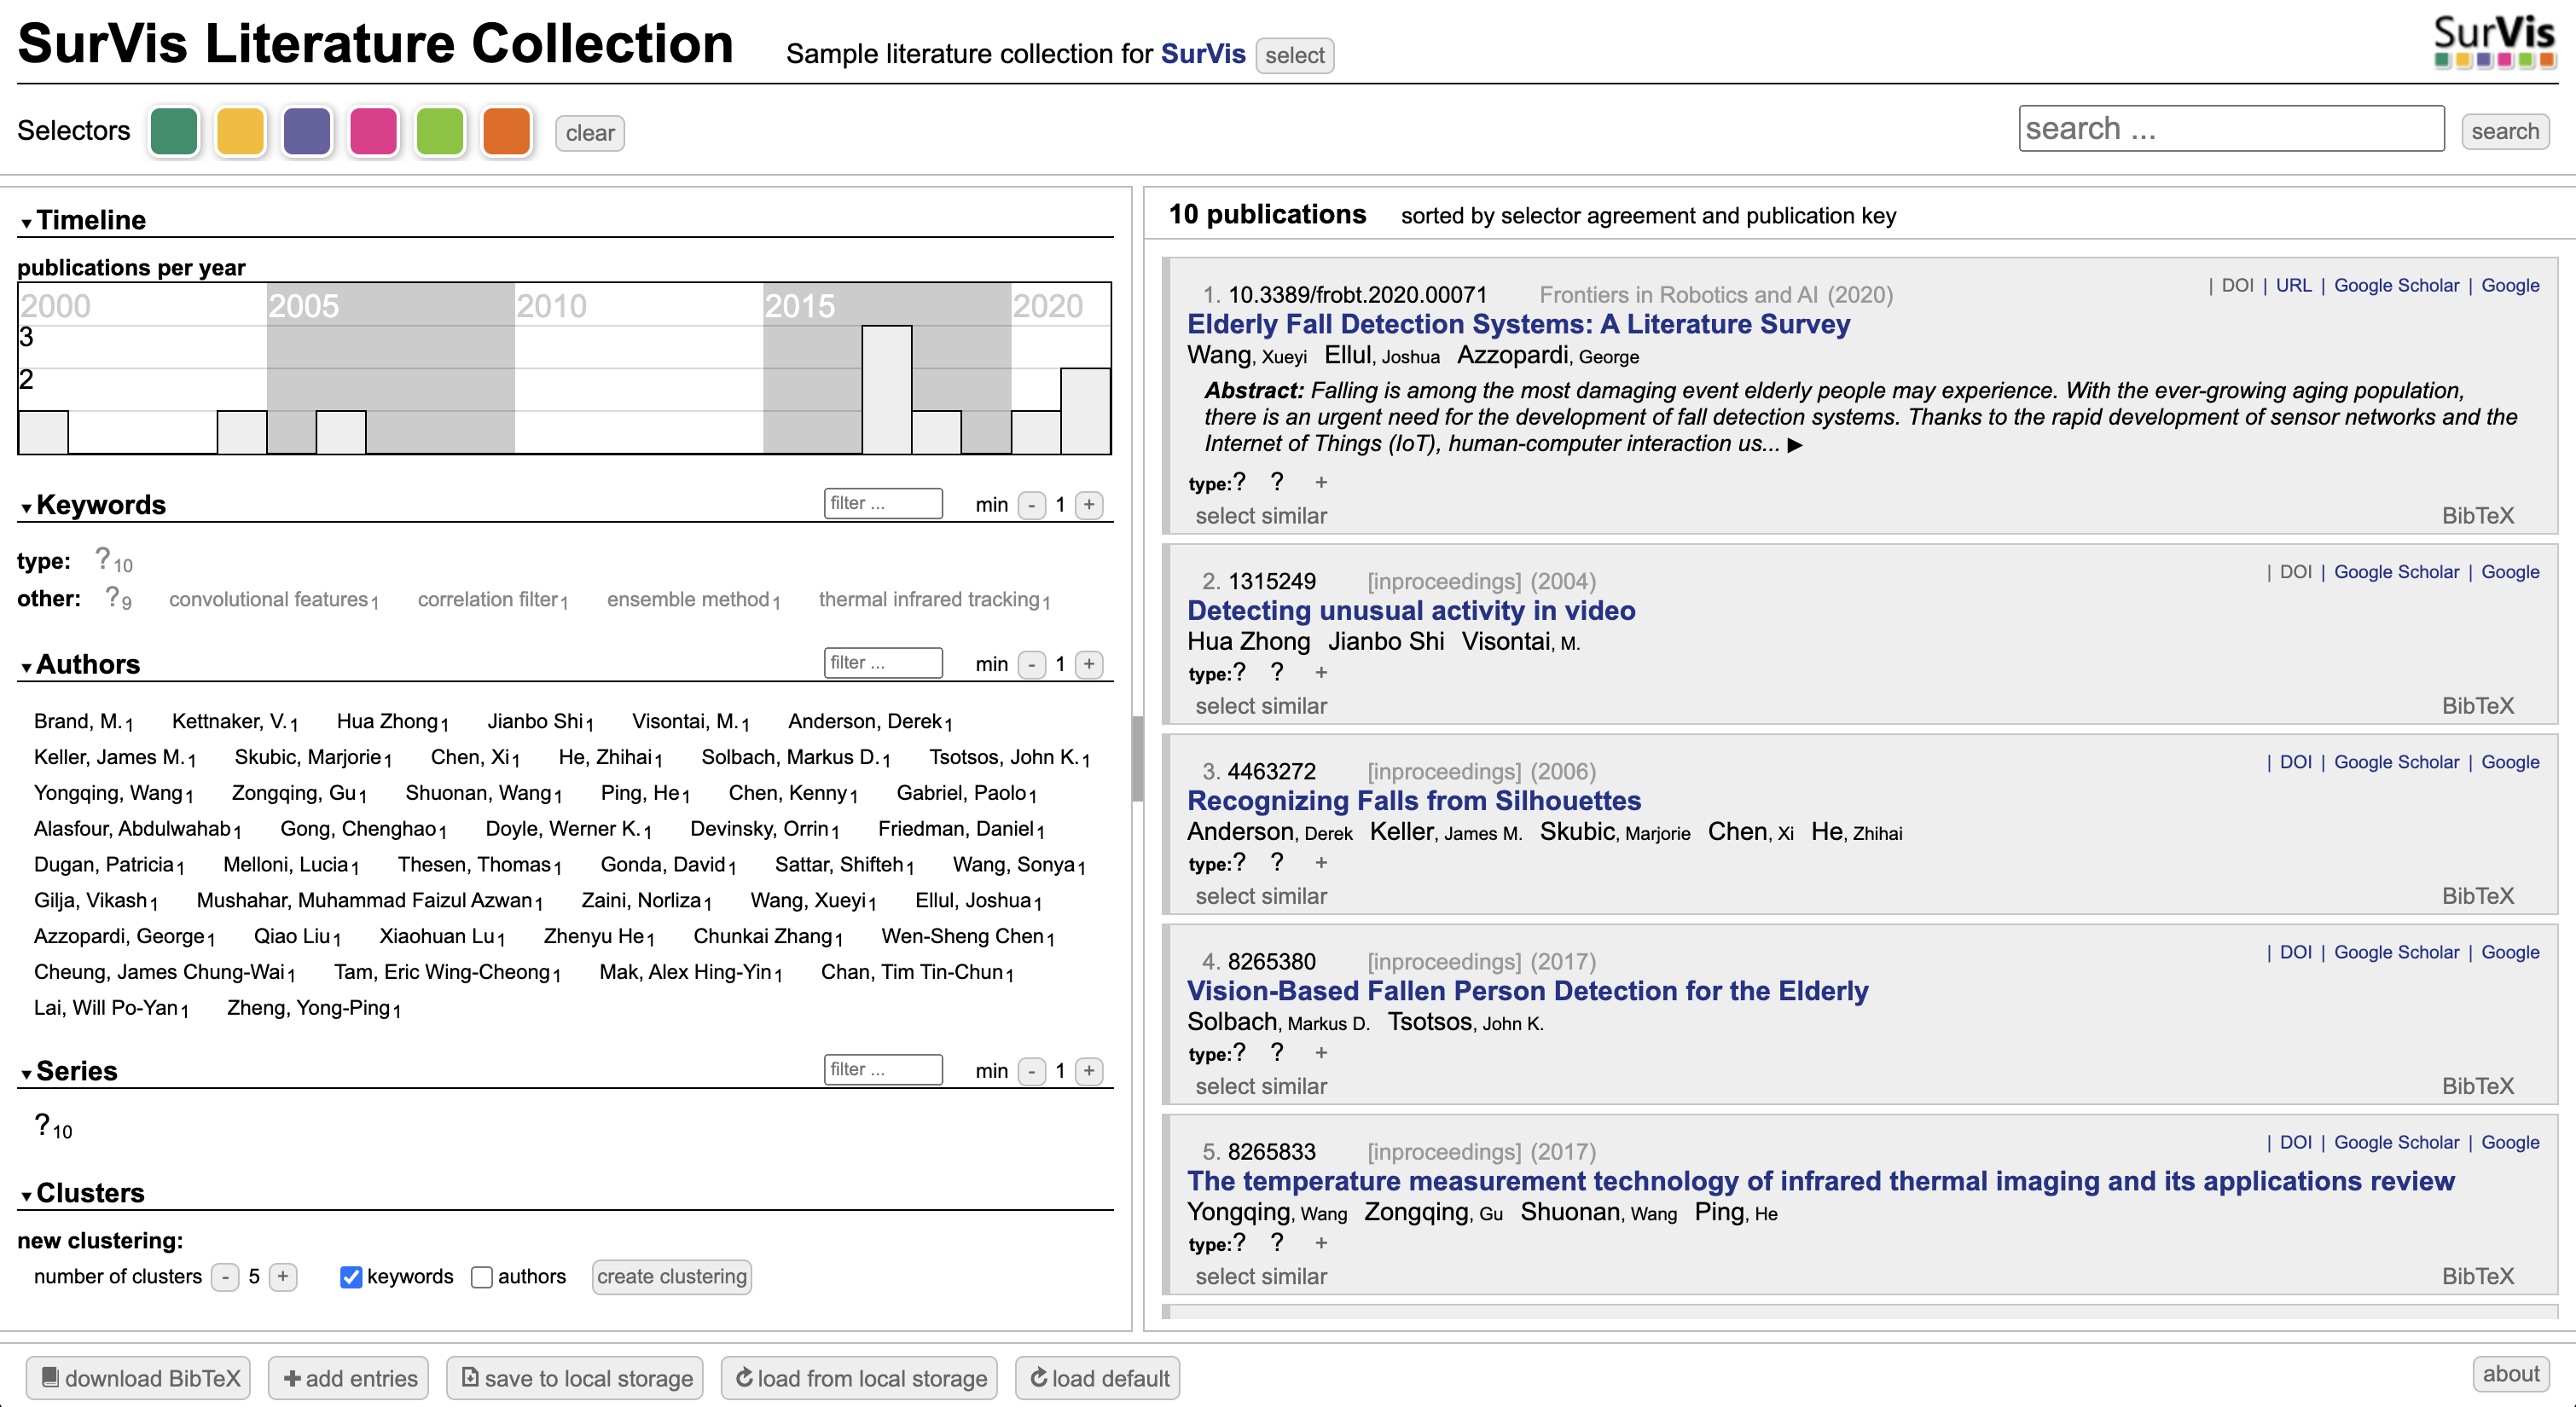
\includegraphics[width=1\textwidth]{survis.pic.jpg}
\caption{Figure4} 
\end{figure}

\noindent abc
\url{abc}

\section{Paper Summaries}

abc
\\ \hspace*{\fill} \\
\textbf{abc}

\noindent abc

\begin{figure}[H]
\centering
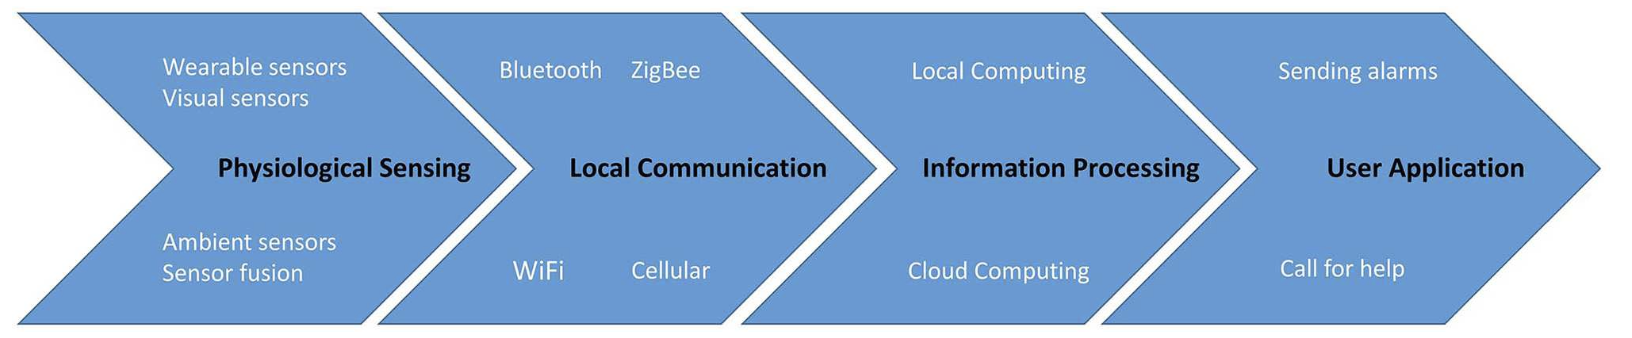
\includegraphics[width=1\textwidth]{Paper1.pic.jpg}
\caption{Figure5} 
\end{figure}

\noindent \textbf{abc}

\noindent abc

\begin{figure}[H]
\centering
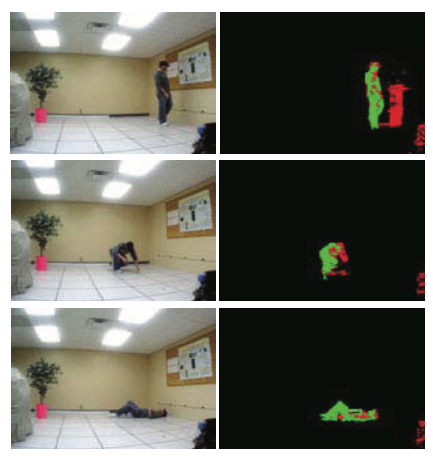
\includegraphics[width=0.7\textwidth]{Paper2.pic.jpg}
\caption{Figure6} 
\end{figure}

\noindent \textbf{abc}

\noindent abc

\begin{figure}[H]
\centering
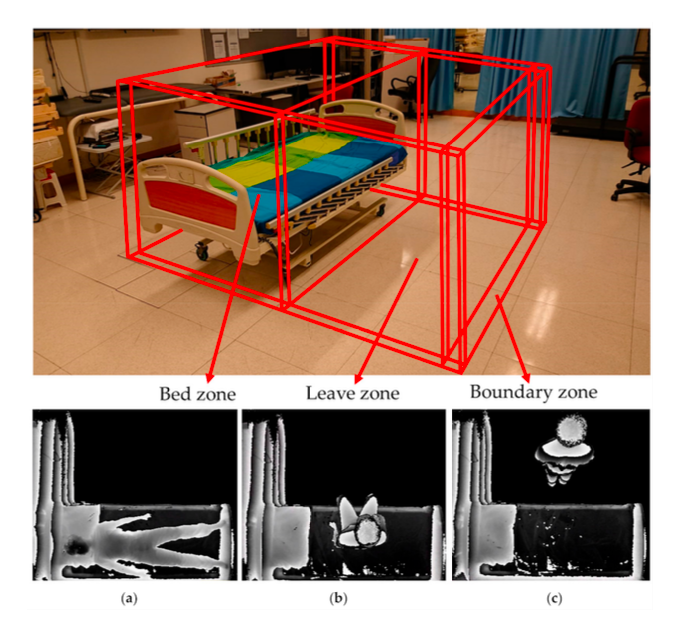
\includegraphics[width=0.7\textwidth]{Paper3.pic.jpg}
\caption{Figure7} 
\end{figure}

\noindent \textbf{abc}

\noindent abc

\begin{figure}[H]
\centering
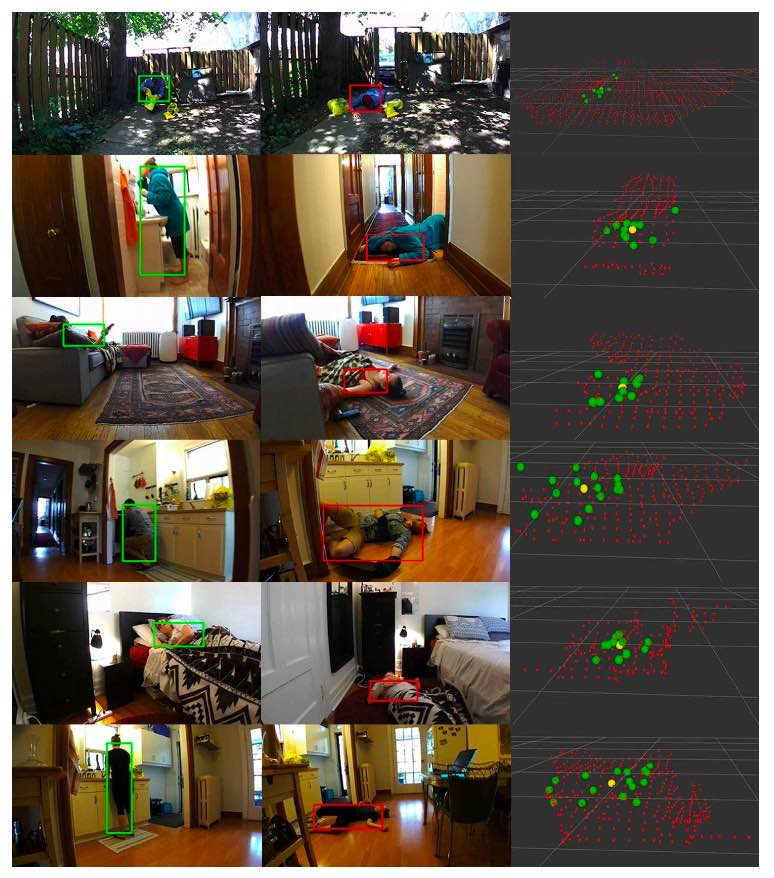
\includegraphics[width=0.7\textwidth]{Paper4.pic.jpg}
\caption{Figure8} 
\end{figure}

\noindent \textbf{abc}

\noindent abc

\begin{figure}[H]
\centering
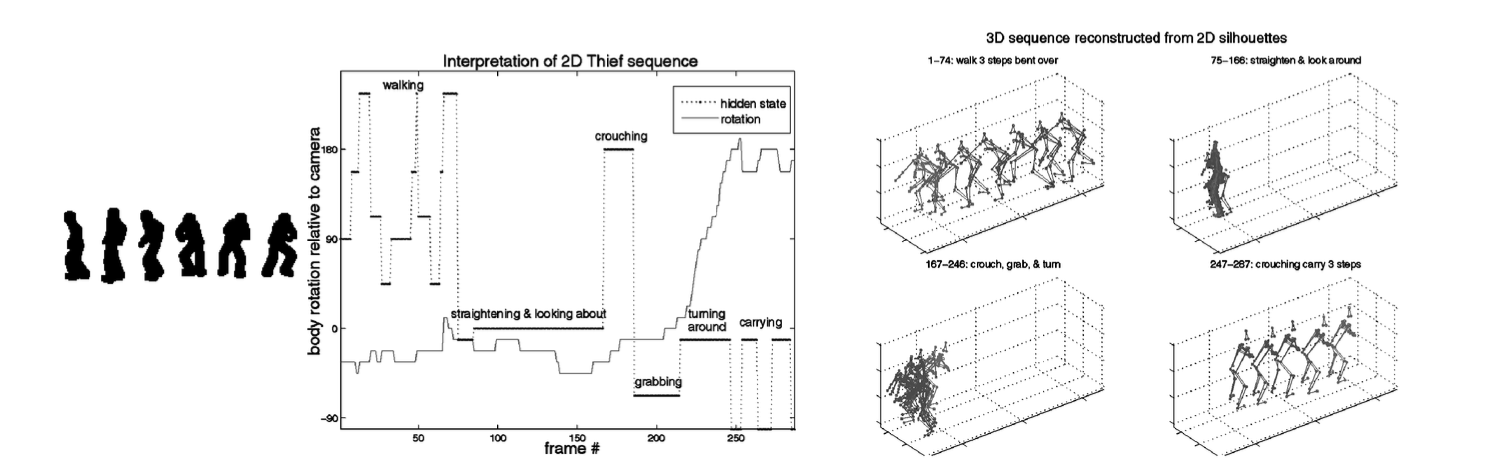
\includegraphics[width=0.7\textwidth]{Paper5.pic.jpg}
\caption{Figure9} 
\end{figure}

\noindent \textbf{abc}

\noindent abc

\begin{figure}[H]
\centering
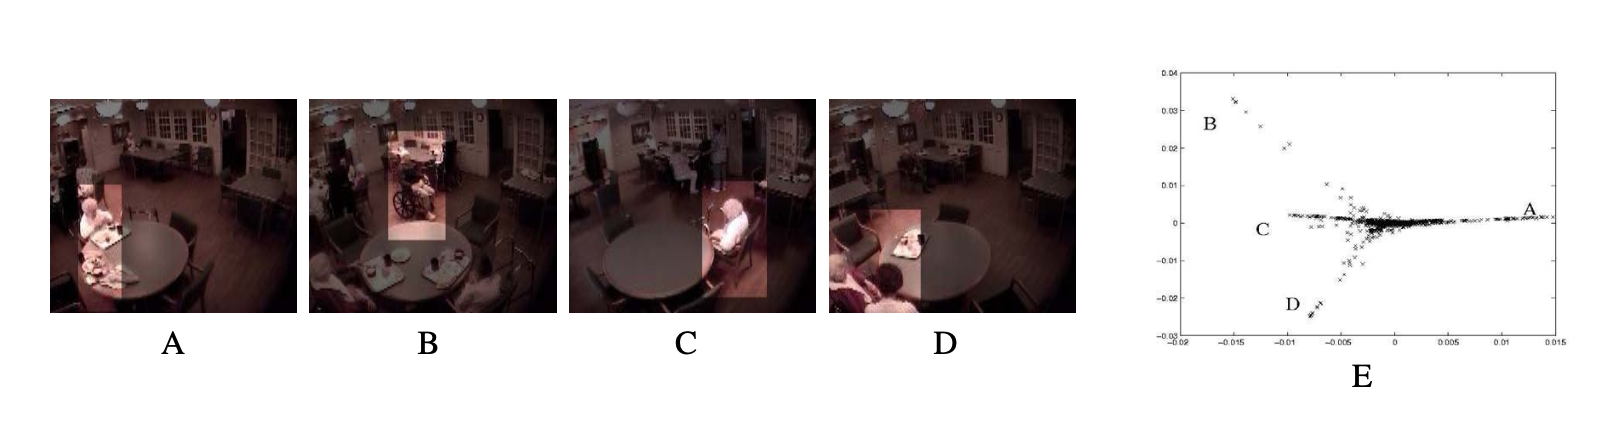
\includegraphics[width=0.7\textwidth]{Paper6.pic.jpg}
\caption{Figure10} 
\end{figure}

\noindent \textbf{abc}

\noindent abc

\begin{figure}[H]
\centering
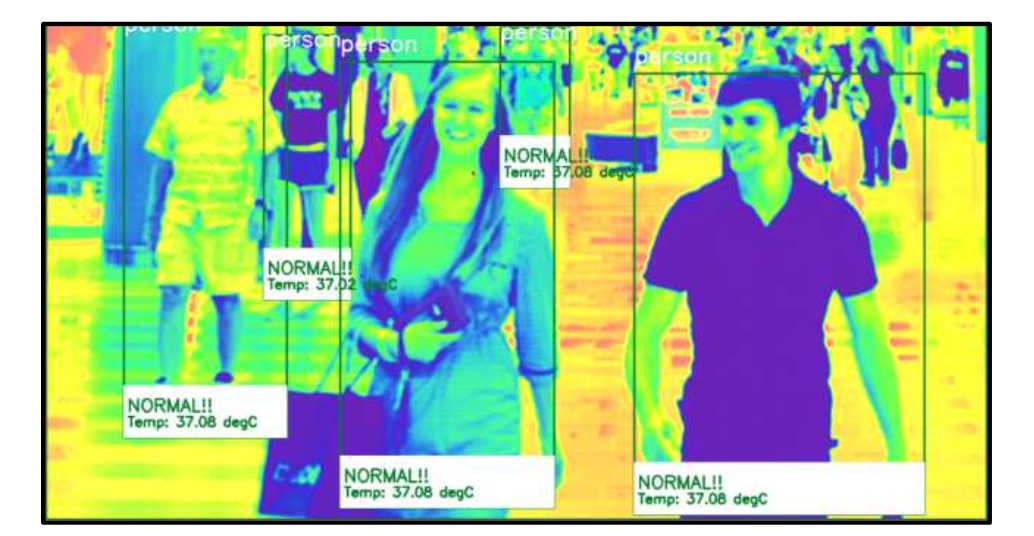
\includegraphics[width=0.7\textwidth]{Paper7.pic.jpg}
\caption{Figure11} 
\end{figure}

\noindent \textbf{abc}

\noindent abc

\begin{figure}[H]
\centering
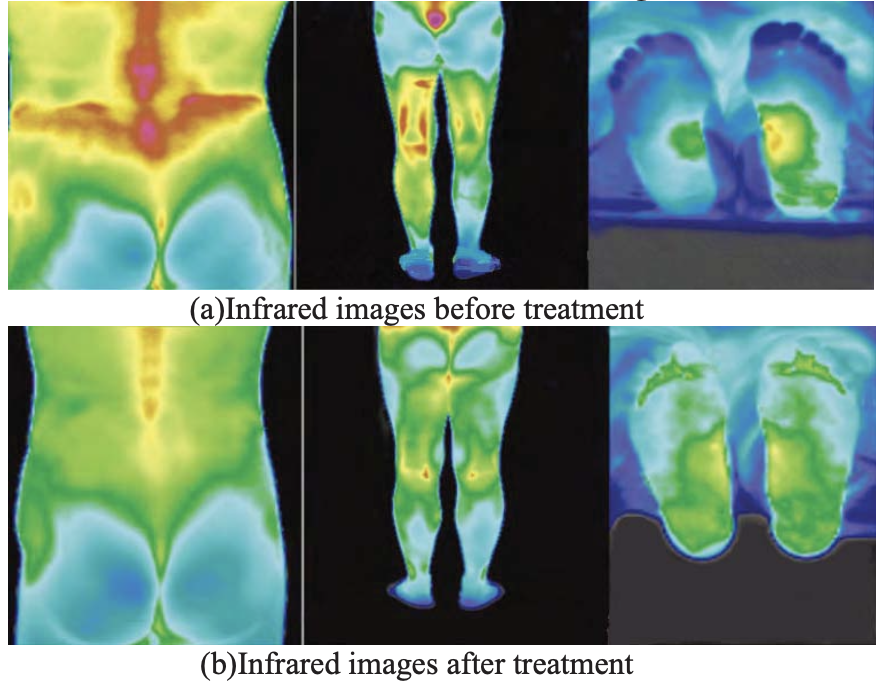
\includegraphics[width=0.7\textwidth]{Paper8.pic.jpg}
\caption{Figure12} 
\end{figure}
    
\noindent \textbf{abc}

\noindent abc

\begin{figure}[H]
\centering
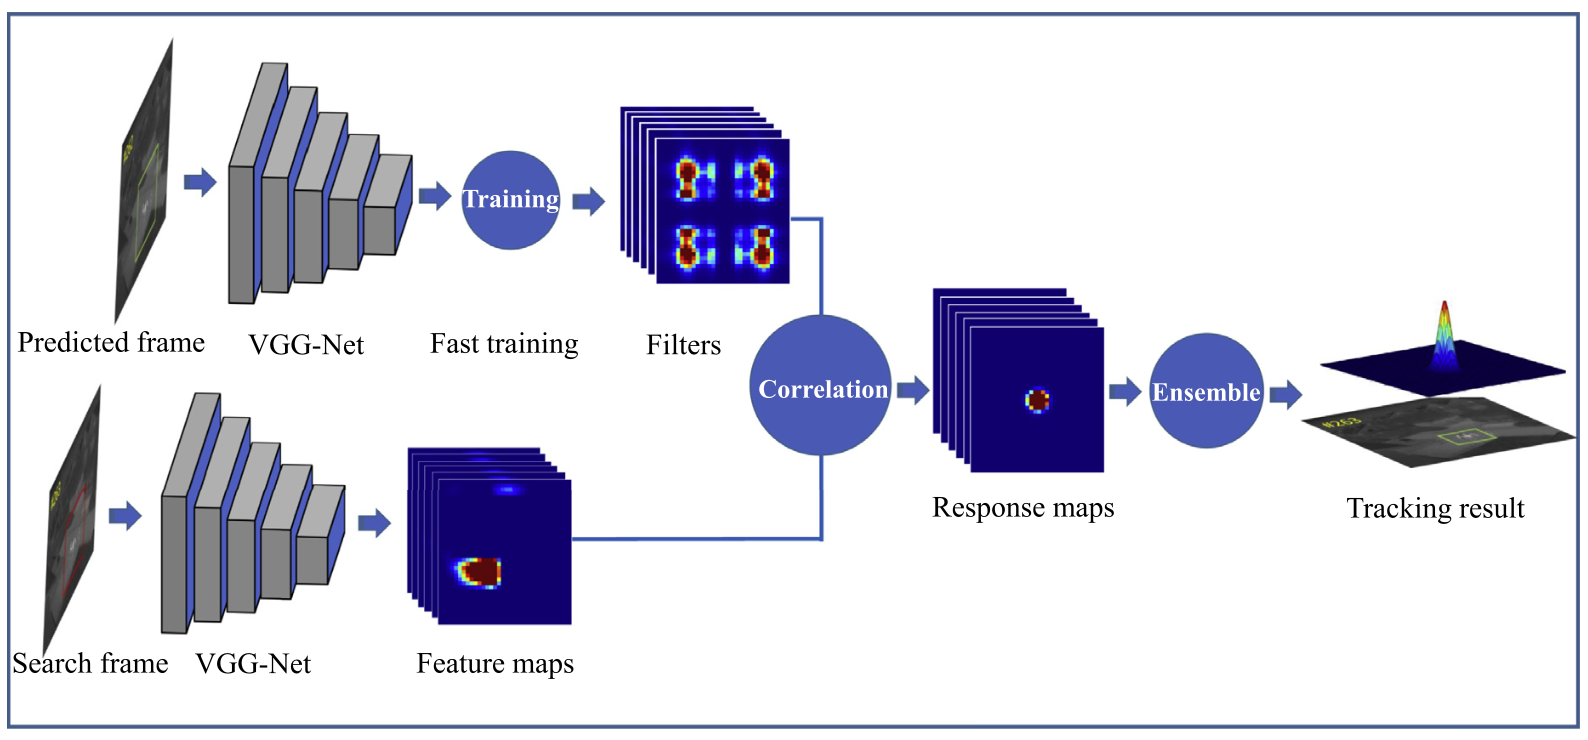
\includegraphics[width=0.7\textwidth]{Paper9.pic.jpg}
\caption{Figure13} 
\end{figure}

\noindent \textbf{abc}

\noindent abc

\begin{figure}[H]
\centering
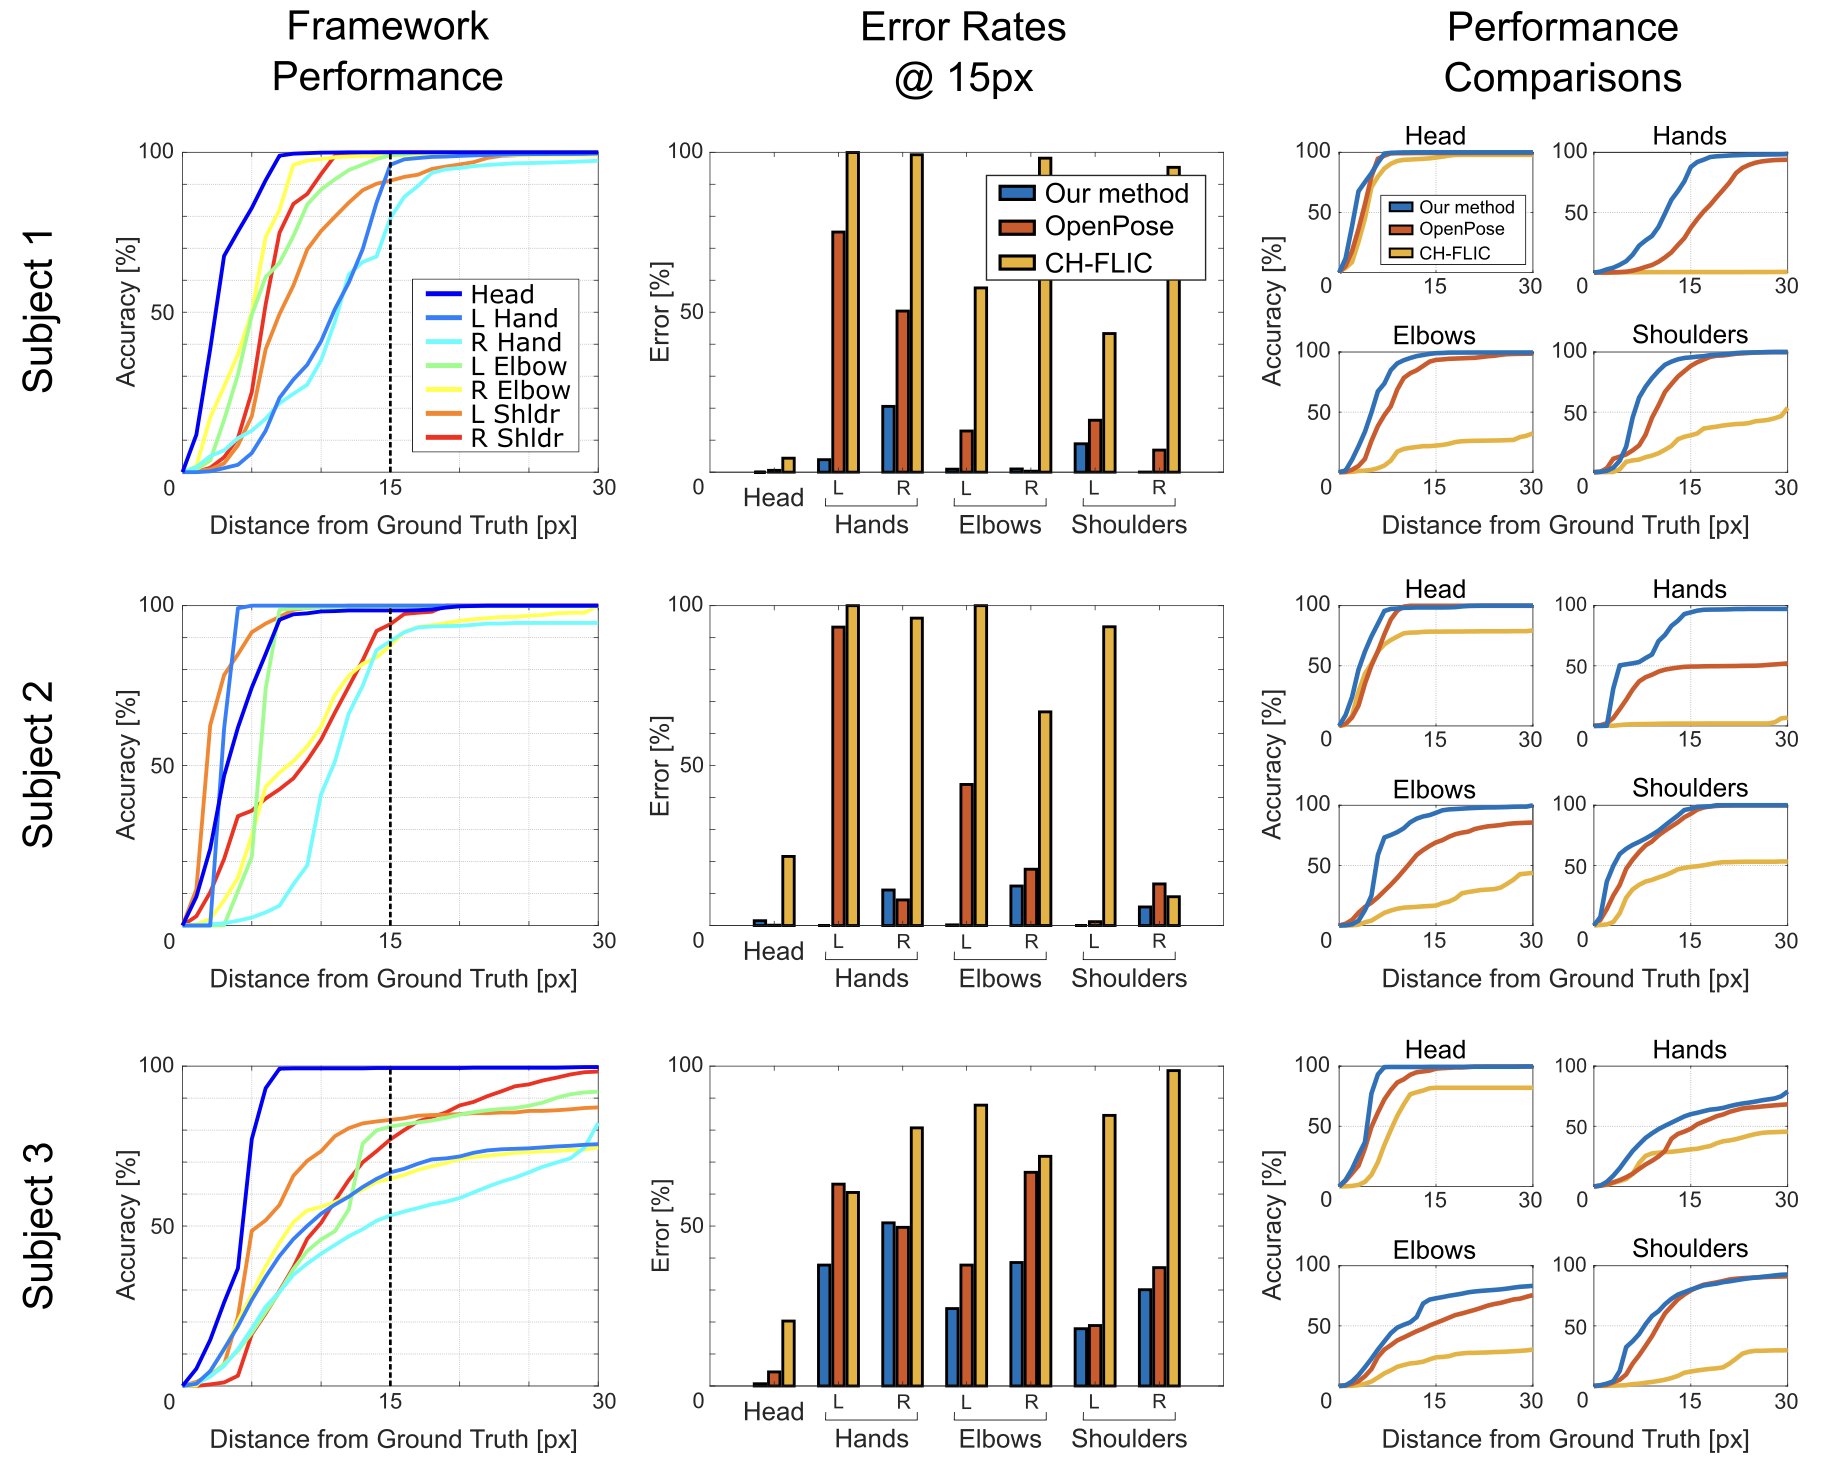
\includegraphics[width=0.7\textwidth]{Paper10.pic.jpg}
\caption{Figure14} 
\end{figure}

\newpage
\section{References}
abc

\noindent abc

\end{document}


